\section{Results}

Our primary evaluation was on Spark and System-X. Both of these systems were
mostly evaluated in stand-alone mode because of issues with System-X (further
discussed in Section~\ref{ssec:sysx-dist}). This section covers the two primary
benchmarks that we ran on both systems (Sections~\ref{ssec:spark1}
and~\ref{ssec:sysx1}) and some graphs of our results and lastly covers some
evaluation of the scalability of spark distributed
(Section~\ref{ssec:spark-dist1}).

\subsection{Spark}
\label{ssec:spark1}

\begin{figure}[t]
\centering
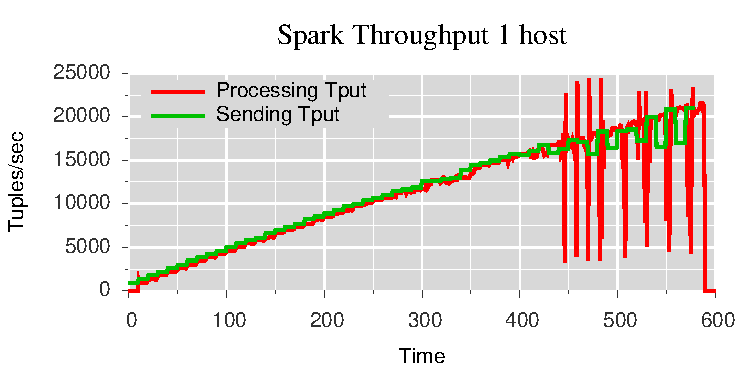
\includegraphics[width=1\linewidth]{figures/sp1_tput.pdf}
\caption{Throughput/Time for a single Spark host running word count. We sent 100B tuples at a
slowly ramped up rate from 1K tuples/sec to 30k tuples/sec with a step size of
500 tuples/sec. The sending rate remained constant for 10 seconds before
transitioning to the next throughput.}
\label{fig:sp1-tput}
\end{figure}

\begin{figure}[t]
\centering
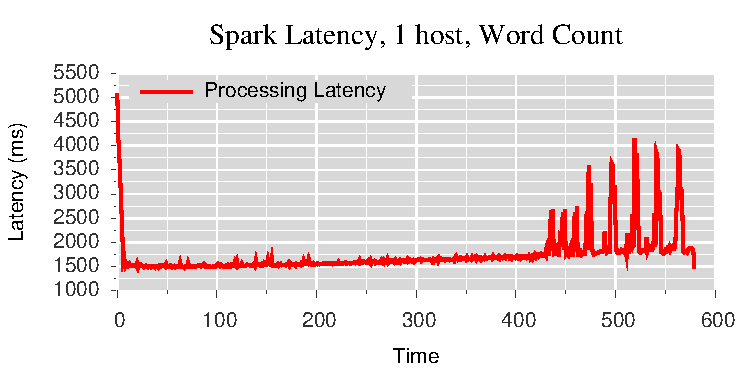
\includegraphics[width=1\linewidth]{figures/sp1_latency.pdf}
\caption{Average latency to process tuples for a single Spark host. Similar to
Figure~\ref{fig:sb1-tput} we sent 100B tuples at a slowly ramped up rate from 1K
tuples/sec to 30k tuples/sec with a step size of 500 tuples/sec. The sending
rate remained constant for 10 seconds before transitioning to the next
throughput. The astute reader will notice that the latency spike in this graph
occurs at the same time as the loss in throughput consistency in
Figure~\ref{fig:sp1-tput}.}
\label{fig:sp1-latency}
\end{figure}

For Spark Streaming we found that our benchmarking methodology finally worked
fairly decently once we were able to measure throughput, latency and fully
saturate the system through tuple generation. Figure~\ref{fig:sp1-tput}
and~\ref{fig:sp1-latency} show the throughput and latency for a word count job. These
figures show that as the sending rate of the tuple generator increases we
finally saturate the system around the 450th time step and at 17,500 tuples per
second. A similar pattern is seem in Figure~\ref{fig:sp1-latency} where around
the 450th time step we see latency spike and never fully recover. 

One interesting note about Figure~\ref{fig:sp1-tput} is that the green line
(sending throughput) roughly matches the received throughput between time step
0 and 450, but time greater than 450 the throughput begins to dip. After
careful thought we concluded that this is because Spark is not draining its TCP
receive buffer fast enough, which is causing the TCP sender to wait for Spark
to catch up before it can send more tuples. This was determined by ensuring
that the tuple generator's TCP sender socket's flag was set to MSG\_WAITALL in
conjunction with Python's sendall function~\cite{python-sockets}. This caused
the sending socket to fully flush all its bytes when it wrote to the socket,
which means if the receiver was already full the send would just have to sit
there waiting, thus drop its overall throughput.


\begin{figure}[t]
\centering
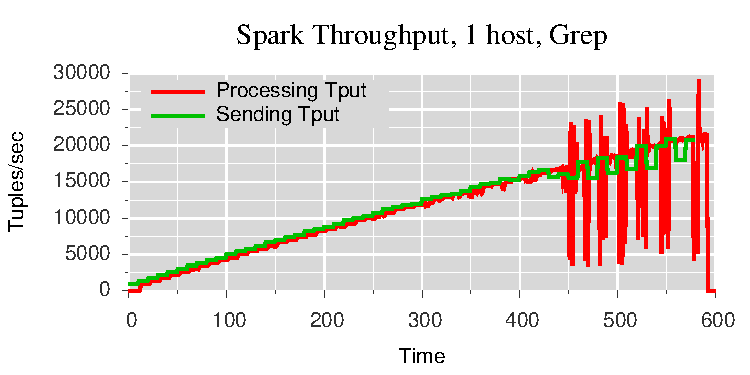
\includegraphics[width=1\linewidth]{figures/sp2_tput.pdf}
\caption{Throughput/Time for a single Spark host, running grep. We sent 100B tuples at a
slowly ramped up rate from 1K tuples/sec to 30k tuples/sec with a step size of
500 tuples/sec. The sending rate remained constant for 10 seconds before
transitioning to the next throughput.}
\label{fig:sp2-tput}
\end{figure}

\begin{figure}[t]
\centering
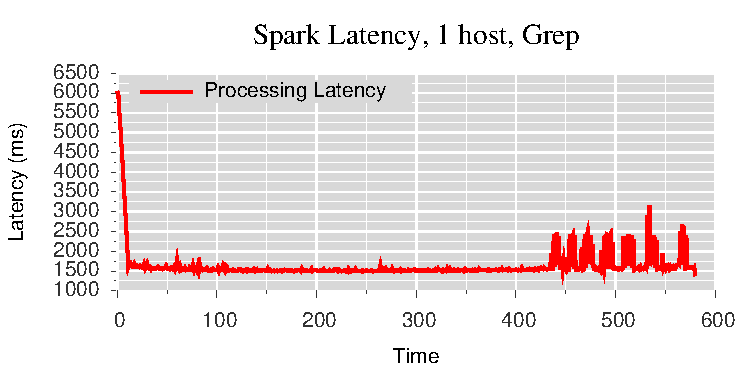
\includegraphics[width=1\linewidth]{figures/sp2_latency.pdf}
\caption{Average latency to process tuples for a single Spark host. Similar to
Figure~\ref{fig:sb1-tput} we sent 100B tuples at a slowly ramped up rate from 1K
tuples/sec to 30k tuples/sec with a step size of 500 tuples/sec. The sending
rate remained constant for 10 seconds before transitioning to the next
throughput. The astute reader will notice that the latency spike in this graph
occurs at the same time as the loss in throughput consistency in
Figure~\ref{fig:sb1-tput}.}
\label{fig:sp2-latency}
\end{figure}

In a similar sense as the word count graphs we also have grep benchmark
results.  We evaluate the system under the same metric, tuple throughput and
latency, which can be seen in Figures~\ref{fig:sp2-tput}
and~\ref{fig:sp2-latency}. We see similar patterns in terms of when the system
cannot handle any higher tuple throughput, around the 450th time step we see
the throughput's values oscillate. Similarly to the word count graphs you can
see the sending throughput also starts oscillating slightly because of the
previously mentioned tight relationship between the TCP sender and receiver.

\subsection{System-X}
\label{ssec:sysx1}

\begin{figure}[t]
\centering
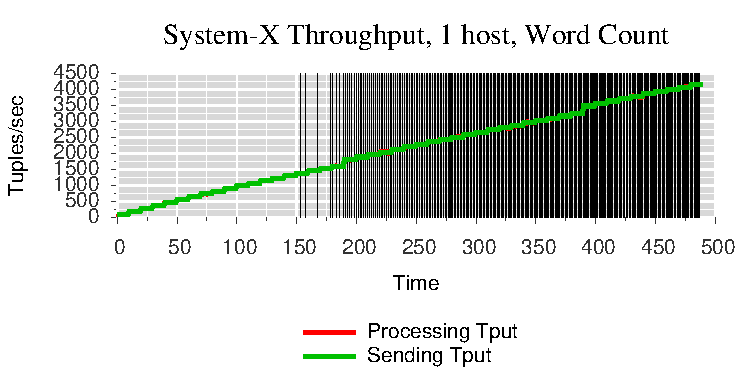
\includegraphics[width=1\linewidth]{figures/sb1_tput.pdf}
\caption{System-X word count. The black vertical bars represent System-X producing errors relating to it unable to transform the bytes in its internal buffer to a tuple.}
\label{fig:sb1-tput}
\end{figure}

\begin{figure}[t]
\centering
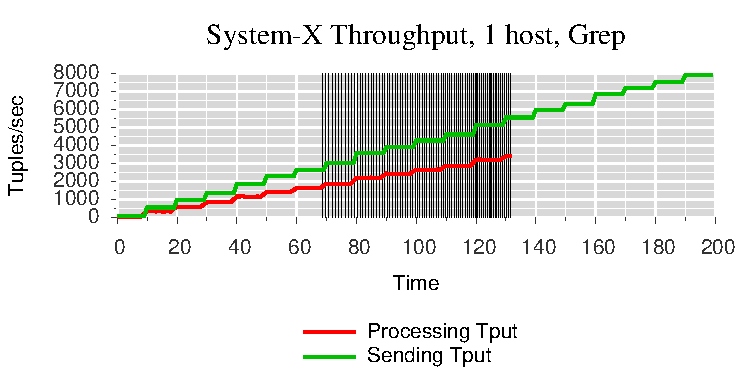
\includegraphics[width=1\linewidth]{figures/sb2_tput.pdf}
\caption{System-X grep. Around time step 130 System-X froze and would not report anymore results but somehow kept the TCP connection with the tuple generator alive since it was happy to keep receiving tuples but dropping them on the floor.}
\label{fig:sb2-tput}
\end{figure}

Evaluating System-X was tricky, since its processing is much different than
Spark. We re-created the word count and grep benchmarks in System-X and they
performed okay but not nearly as good as Spark. System-X also has a much
different failure condition. When System-X begins to get over saturated it
starts raising buffer exceptions on the client. We saw various strange behavior
by System-X while trying to overload it which can be broken down into 3
non-mutually-exclusive categories: hundreds of buffer exceptions raised, locked
up client application and simply dropping tuples. We found the buffer
exceptions to be the most interesting since they had an associated timestamp
and we could correlate them with other events and graph them. As seen in 
Figures~\ref{fig:sb1-tput} and~\ref{fig:sb2-tput}, the black vertical lines
indicate buffer exception events that were produced by the client.

\subsection{Spark Distributed}
\label{ssec:spark-dist1}

\begin{figure}[t]
\centering
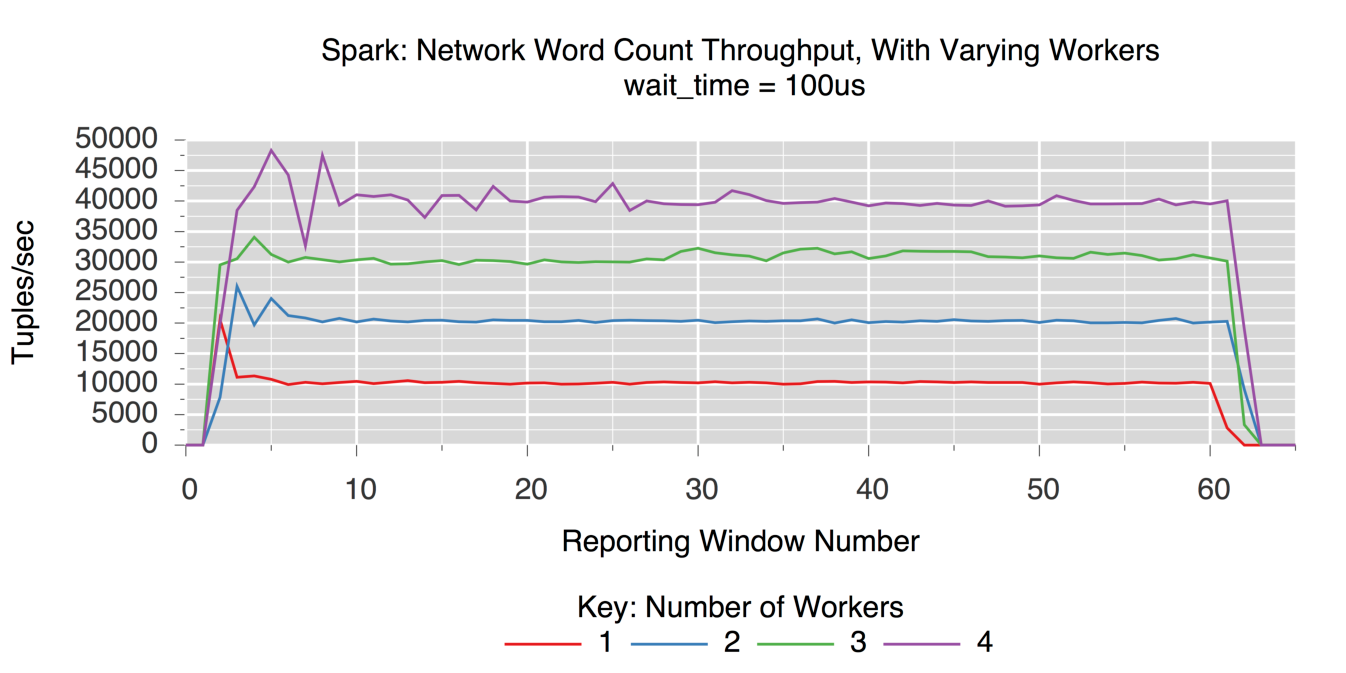
\includegraphics[width=1\linewidth]{figures/spark-wc-dist.pdf}
\caption{Spark distributed, word count}
\label{fig:spark-wc-dist}
\end{figure}


\begin{figure}[t]
\centering
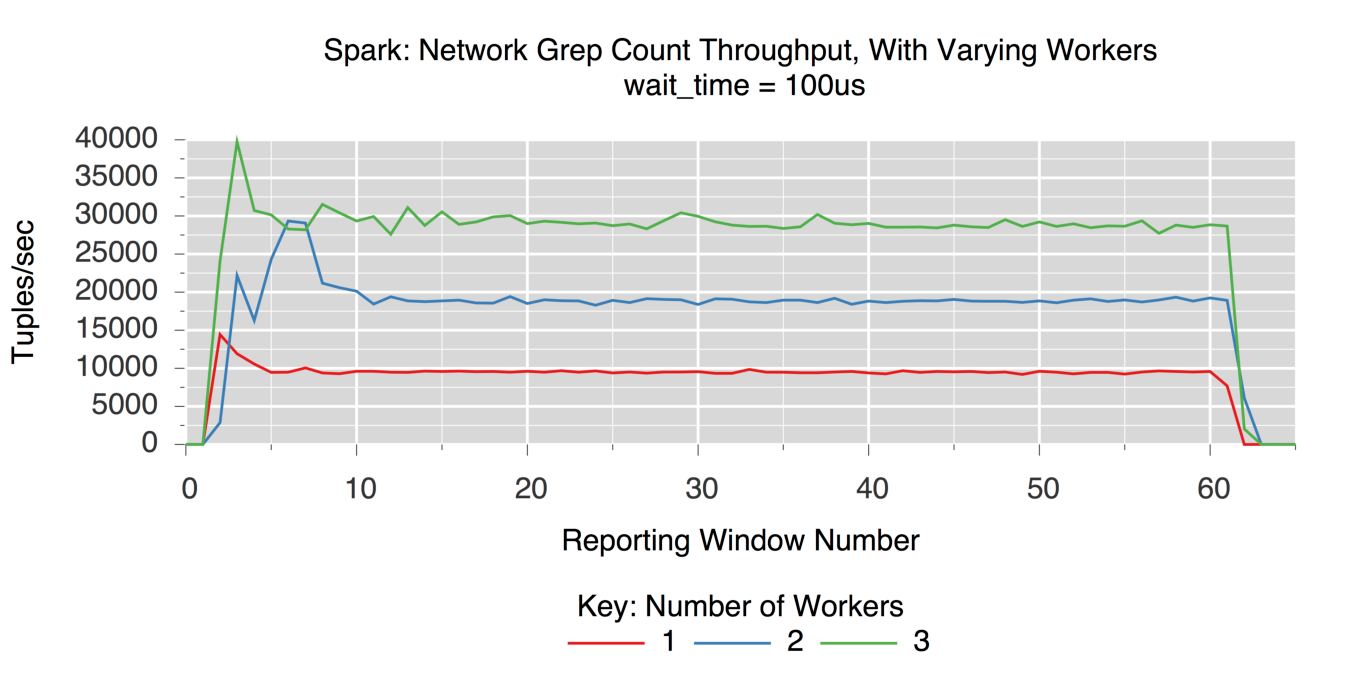
\includegraphics[width=1\linewidth]{figures/spark-grep-dist.pdf}
\caption{Spark distributed, grep}
\label{fig:spark-grep-dist}
\end{figure}




